\section{Аналитический раздел}
В данном разделе проведена формализация задачи и формализация данных. Был проведен обзор существующих решений, используемых для проведения футбольных турниров. Также были проанализированы различные модели баз данных, включая дореляционные, реляционные и постреляционные. Кроме того, были описаны типы пользователей, которые будут взаимодействовать с разработанной базой данных.
\subsection{Формализация задачи}
Необходимо спроектировать базу данных для хранения информации о пользователях, командах, странах, турнирах и матчах для проведения футбольных турниров. Требуется разработать Desktop-приложение, предоставляющее интерфейс для просмотра, добавления, изменения и удаления информации, хранящейся в базе данных. Необходимо реализовать три вида ролей --- гость, авторизованный пользователь и администратор.

\subsection{Анализ существующих решений}
Среди решений, предоставляющих функционал для проведения футбольных турниров, были выделены 3 аналога:
\begin{itemize}
    \item oball.ru \cite{oball};
    \item sportcup.org \cite{sportcup};
    \item tlab.pro \cite{tlab}.
\end{itemize}

Для сравнения были выбраны следующие критерии:
\begin{enumerate}
    \item Возможность просмотра турниров других пользователей.
    \item Возможность создания турнира с уже существующими командами.
    \item Возможность просмотра информации о стране проведения турниров.
\end{enumerate}

В таблице \ref{decisions} представлено сравнение по вышеупомянутым критериям.

\begin{table}[ht!]
	\centering
	\caption{Существующие решения поставленной задачи}
	\label{decisions}
	\begin{tabular}{|p{2.6cm}|p{3cm}|p{3cm}|p{3cm}|}
			\hline
			\textbf{Критерий} & \textbf{oball.ru} & \textbf{sportcup.org} & \textbf{tlab.pro}\\
			\hline
			\textbf{1} & + & + & +\\
			\hline
			\textbf{2} & + & - & -\\
			\hline
			\textbf{3} & - & -& -\\
			\hline
	\end{tabular}
\end{table}

Таким образом, среди представленных решений нет ни одного проекта, позволяющего просматривать информацию о стране проведения турниров. Кроме того, только в одном проекте есть возможность создания турнира с уже существующими командами. Разрабатываемое программное обеспечение будет предоставлять данный функционал.

\subsection{Анализ моделей баз данных}

База данных --- это самодокументированное собрание интегрированных записей. Модель базы данных определяет логическую структуру базы данных. Существует три основных типа модели баз данных:
\begin{enumerate}
    \item Дореляционные.
    \item Реляционные.
    \item Постреляционные.
\end{enumerate}

К дореляционным моделям данных относятся иерархические и сетевые модели баз данных.

Информация в иерархической модели организована по принципу древовидной структуры, в виде отношений «предок-потомок» \cite{ierar}. Каждая запись может иметь не более одной родительской записи и несколько подчиненных. Связи записей реализуются в виде физических указателей с одной записи на другую. Основной недостаток иерархической модели — невозможность реализовать отношения «многие-ко-многим», а также ситуации, когда запись имеет несколько предков.

Сетевая модель отличается от иерархической тем, что у потомка может быть любое количество предков.

Реляционная модель предназначена для хранения и организации точек данных с заданными отношениями для быстрого доступа. Данные в реляционных базах данных упорядочиваются в виде таблиц, которые содержат информацию о каждой сущности и представляют заданные заранее категории с помощью строк и столбцов \cite{relat}. Такое структурирование данных повышает эффективность и гибкость доступа. Кроме того, реляционная модель наиболее эффективно поддерживает целостность данных во всех приложениях и копиях (экземплярах) базы данных. 

Постреляционная модель базы данных представляет собой расширенную реляционную модель, снимающую ограничение неделимости данных, хранящихся в записях таблиц. Постреляционная модель допускает наличие множественных значений в полях данных. Значения таких полей могут быть разделены на несколько подзначений, которые считаются отдельными записями в таблице. Главным недостатком этой модели является сложность решения проблемы обеспечения целостности и непротиворечивости хранимых данных.

В качестве модели базы данных была выбрана реляционная модель, поскольку она обеспечивает целостность данных, эффективность и гибкость доступа к данным, а также исключает дублирование данных.

\subsection{Формализация данных}
Разрабатываемая база данных должна содержать информацию о пользователях, командах, странах, турнирах и матчах.
В таблице \ref{info} представлены категории данных в БД и информация о них.

\begin{table}[ht!]
	\centering
	\caption{Категории данных в БД и информация о них}
	\label{info}
	\begin{tabular}{|p{4cm}|p{10cm}|}
			\hline
			\textbf{Категория} & \textbf{Информация}\\
			\hline
			Пользователь & Id пользователя, логин, hash пароля, права доступа \\
			\hline
			Команда & Id команды, название, Id страны базирования \\
			\hline
			Страна & Id страны, название, конфедерация \\
			\hline
            Матч & Id матча, Id турнира, Id домашней команды, Id гостевой команды, голы домашней команды, голы гостевой команды \\
			\hline
            Турнир & Id турнира, название, Id пользователя (создателя), Id страны проведения \\
			\hline
            Связь команды и турнира & Id команды, Id турнира \\
			\hline
	\end{tabular}
\end{table}
\newpage
На рисунке \ref{img:er} представлена ER-диаграмма системы в нотации Чена.
\begin{figure}
  \centering
  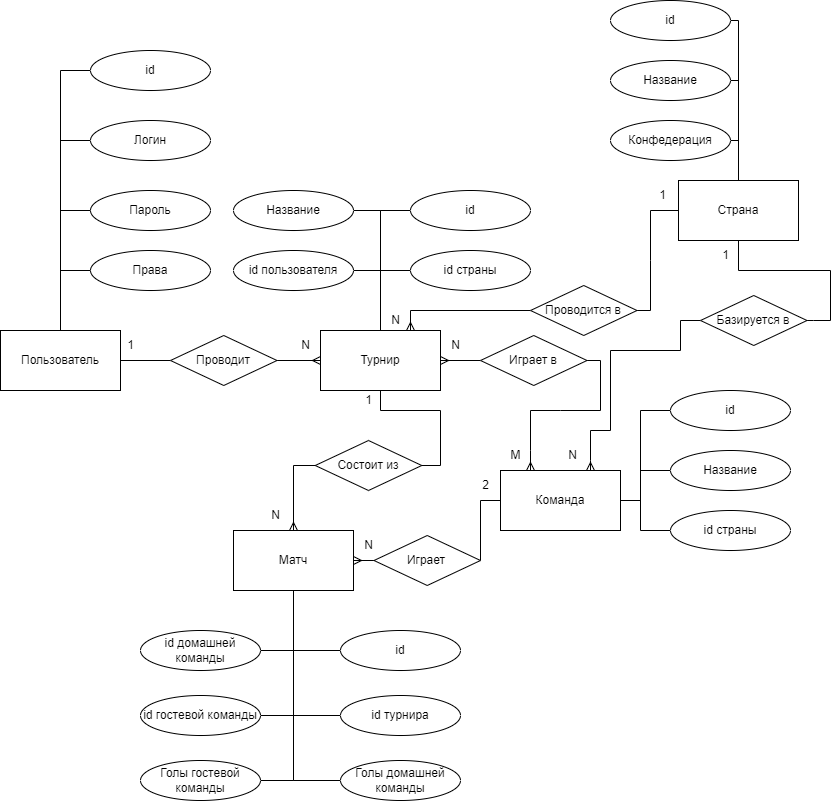
\includegraphics[scale=0.5]{inc/er}
  \caption{ER-диаграмма системы в нотации Чена}
  \label{img:er}
\end{figure}

\subsection{Описание пользователей}
Было выделено три категории пользователей --- гость, авторизованный пользователь и администратор.

Гость может просматривать информацию о пользователях, командах, странах, турнирах (в том числе турнирную таблицу и результаты матчей), а также зарегистрироваться или авторизоваться.
\begin{figure}
  \centering
  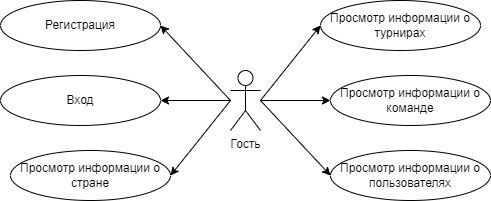
\includegraphics[scale=0.7]{inc/ppo}
  \caption{Use-case диаграмма для гостя}
  \label{img:ppo}
\end{figure}

Авторизованный пользователь, кроме просмотра информации, может создавать команды и турниры, а также
редактировать информацию о матчах своих турниров.
\begin{figure}
  \centering
  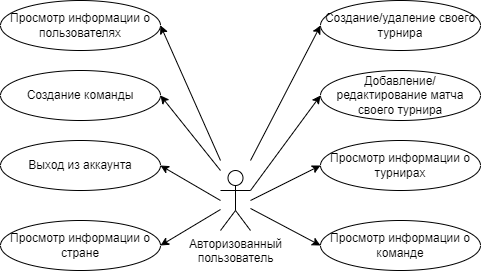
\includegraphics[scale=0.7]{inc/ppo1}
  \caption{Use-case диаграмма для авторизованного пользователя}
  \label{img:ppo1}
\end{figure}

В качестве дополнительного функционала администратор может добавлять страны и изменять права пользователей.
\begin{figure}
  \centering
  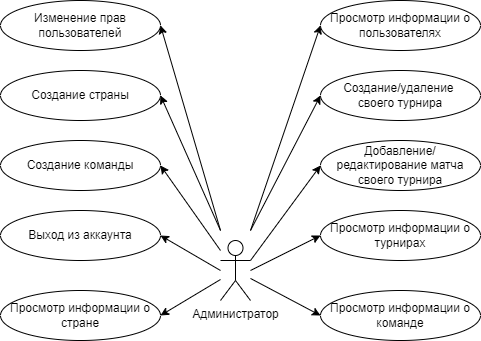
\includegraphics[scale=0.7]{inc/ppo2}
  \caption{Use-case диаграмма для администратора}
  \label{img:ppo2}
\end{figure}

\subsection*{Вывод}
В данном разделе была проведена формализация задачи, формализация данных, анализ существующих решений и анализ моделей баз данных и описаны типы пользователей. В качестве модели базы данных была выбрана реляционная модель.